
%% 2-column papers and preprints
\documentclass[journal abbreviation, manuscript]{copernicus}

%% Journal abbreviations (please use the same for preprints and final revised papers)


%% \usepackage commands included in the copernicus.cls:
%\usepackage[german, english]{babel}
%\usepackage{tabularx}
%\usepackage{cancel}
\usepackage{multirow}
%\usepackage{supertabular}
%\usepackage{algorithmic}
%\usepackage{algorithm}
%\usepackage{amsthm}
%\usepackage{float}
%\usepackage{subfig}
%\usepackage{rotating}
\usepackage{pdflscape}
\usepackage{booktabs}
\usepackage{standalone} % Load standalone package

\begin{document}

\title{Supplementary materials to: The Open Global Glacier Data Assimilation Framework (AGILE) v0.1}



\Author[1]{Patrick}{Schmitt}
\Author[1,2]{Fabien}{Maussion}
\Author[3]{Daniel}{Goldberg}
\Author[4]{Philipp}{Gregor}

\affil[1]{Department of Atmospheric and Cryospheric Sciences, University of Innsbruck, Innsbruck, Austria}
\affil[2]{School of Geographical Sciences, University of Bristol, Bristol, United Kingdom}
\affil[3]{School of Geosciences, University of Edinburgh, Edinburgh, United Kingdom}
\affil[4]{Meteorologisches Institut, Ludwig-Maximilians-Universität München, München, Germany}

\correspondence{Patrick Schmitt (patrick.schmitt@uibk.ac.at)}

\runningtitle{TEXT}

\runningauthor{TEXT}

\firstpage{1}

\maketitle

%\noindent\textbf{Contents of this file}
%%%Remove or add items as needed%%%
%\begin{enumerate}
%\item Text S1 to Sx
%\item Figures S1 to S5
%\item Tables S1 to Sx
%\end{enumerate}

\setcounter{figure}{0}
\renewcommand{\figurename}{Figure}
\renewcommand{\thefigure}{S\arabic{figure}}

\renewcommand{\tablename}{Table}
\renewcommand{\thetable}{S\arabic{table}}

% statistics all glaciers and dynamic states
\begin{table}[]
\begin{tabular}{@{}llllll@{}}
\toprule
Glacier geometry & Dynamic state & First guess method & MAD\_BED {[}m{]} & MAD\_V\_1980 {[}1e6 m³{]} & MAD\_V\_2020 {[}1e6 m³{]} \\ \midrule
Aletsch          & retreating    & OGGM               & 8.7              & 3.55                      & 3.8                       \\
                 &               & GlabTop            & 6.4              & 8.87                      & 6.97                      \\ \cmidrule(l){2-6} 
                 & advancing     & OGGM               & 12.7             & 11.28                     & 10.1                      \\
                 &               & GlabTop            & 22.9             & 9.52                      & 10.1                      \\ \cmidrule(l){2-6} 
                 & equilibrium   & OGGM               & 1.5              & 1.88                      & 1.78                      \\
                 &               & GlabTop            & 9                & 5.75                      & 8.15                      \\ \midrule
Artesonraju      & retreating    & OGGM               & 2                & 0.27                      & 0.14                      \\
                 &               & GlabTop            & 6.9              & 0.42                      & 0.2                       \\ \cmidrule(l){2-6} 
                 & advancing     & OGGM               & 0.6              & 0.47                      & 0.15                      \\
                 &               & GlabTop            & 2.3              & 0.69                      & 0.24                      \\ \cmidrule(l){2-6} 
                 & equilibrium   & OGGM               & 0.2              & 0.03                      & 0.03                      \\
                 &               & GlabTop            & 0.7              & 0.17                      & 0.06                      \\ \midrule
Baltoro          & retreating    & OGGM               & 9                & 17.86                     & 22.42                     \\
                 &               & GlabTop            & 73               & 216.3                     & 229.82                    \\ \cmidrule(l){2-6} 
                 & advancing     & OGGM               & 6.7              & 31.26                     & 38.83                     \\
                 &               & GlabTop            & 61.3             & 246.02                    & 270.53                    \\ \cmidrule(l){2-6} 
                 & equilibrium   & OGGM               & 4.7              & 22.2                      & 26.79                     \\
                 &               & GlabTop            & 73.2             & 228.22                    & 246.4                     \\ \midrule
Peyto            & retreating    & OGGM               & 4                & 0.28                      & 0.12                      \\
                 &               & GlabTop            & 4.1              & 0.29                      & 0.17                      \\ \cmidrule(l){2-6} 
                 & advancing     & OGGM               & 5.9              & 0.5                       & 0.62                      \\
                 &               & GlabTop            & 4.5              & 1.34                      & 1.34                      \\ \cmidrule(l){2-6} 
                 & equilibrium   & OGGM               & 0.6              & 0.1                       & 0.09                      \\
                 &               & GlabTop            & 3.8              & 0.61                      & 0.64                      \\ \bottomrule
\end{tabular}
\caption{Performance matrices MAD\_BED, MAD\_V\_1980 and MAD\_V\_2020 for all glacier geometries, all dynamic states and the two used first guess methods.}
\label{tab:sup_fg_statistics}
\end{table}

% number control variables and cpu runtime
\begin{table}[]
\begin{tabular}{ccccc}
\hline
Glacier geometry     & Dynamic state & Number control variables & \begin{tabular}[c]{@{}c@{}}Total CPU runtime \\ per iteration {[}s{]}\end{tabular} & \begin{tabular}[c]{@{}c@{}}CPU runtime only\\ per gradient calculation {[}s{]}\end{tabular} \\ \hline
Aletsch              & retreating    & 120                      & 1.29                                                                               & 0.12                                                                                        \\ \cline{2-5} 
                     & advancing     & 140                      & 2.49                                                                               & 0.23                                                                                        \\ \cline{2-5} 
                     & equilibrium   & 120                      & 1.81                                                                               & 0.23                                                                                        \\ \hline
Artesonraju          & retreating    & 84                       & 1.03                                                                               & 0.08                                                                                        \\ \cline{2-5} 
                     & advancing     & 72                       & 1.24                                                                               & 0.11                                                                                        \\ \cline{2-5} 
                     & equilibrium   & 56                       & 0.75                                                                               & 0.05                                                                                        \\ \hline
Baltoro              & retreating    & 210                      & 1.34                                                                               & 0.11                                                                                        \\ \cline{2-5} 
                     & advancing     & 214                      & 1.78                                                                               & 0.16                                                                                        \\ \cline{2-5} 
                     & equilibrium   & 218                      & 1.47                                                                               & 0.14                                                                                        \\ \hline
Peyto                & retreating    & 72                       & 0.71                                                                               & 0.06                                                                                        \\ \cline{2-5} 
                     & advancing     & 104                      & 1.03                                                                               & 0.08                                                                                        \\ \cline{2-5} 
\multicolumn{1}{l}{} & equilibrium   & 94                       & 0.71                                                                               & 0.05                                                                                        \\ \hline
\end{tabular}
\caption{Showing the number of control variables and the CPU runtime for one total iteration (forward model run and gradient calculation) and the CPU runtime only for the gradient calculation for all glacier geometries and dynamic glacier states.}
\label{tab_sup:number_control_vars_cpu_runtime}
\end{table}

% geometry creation plots and first guess bed
\begin{landscape}
\begin{figure}
    \centering
    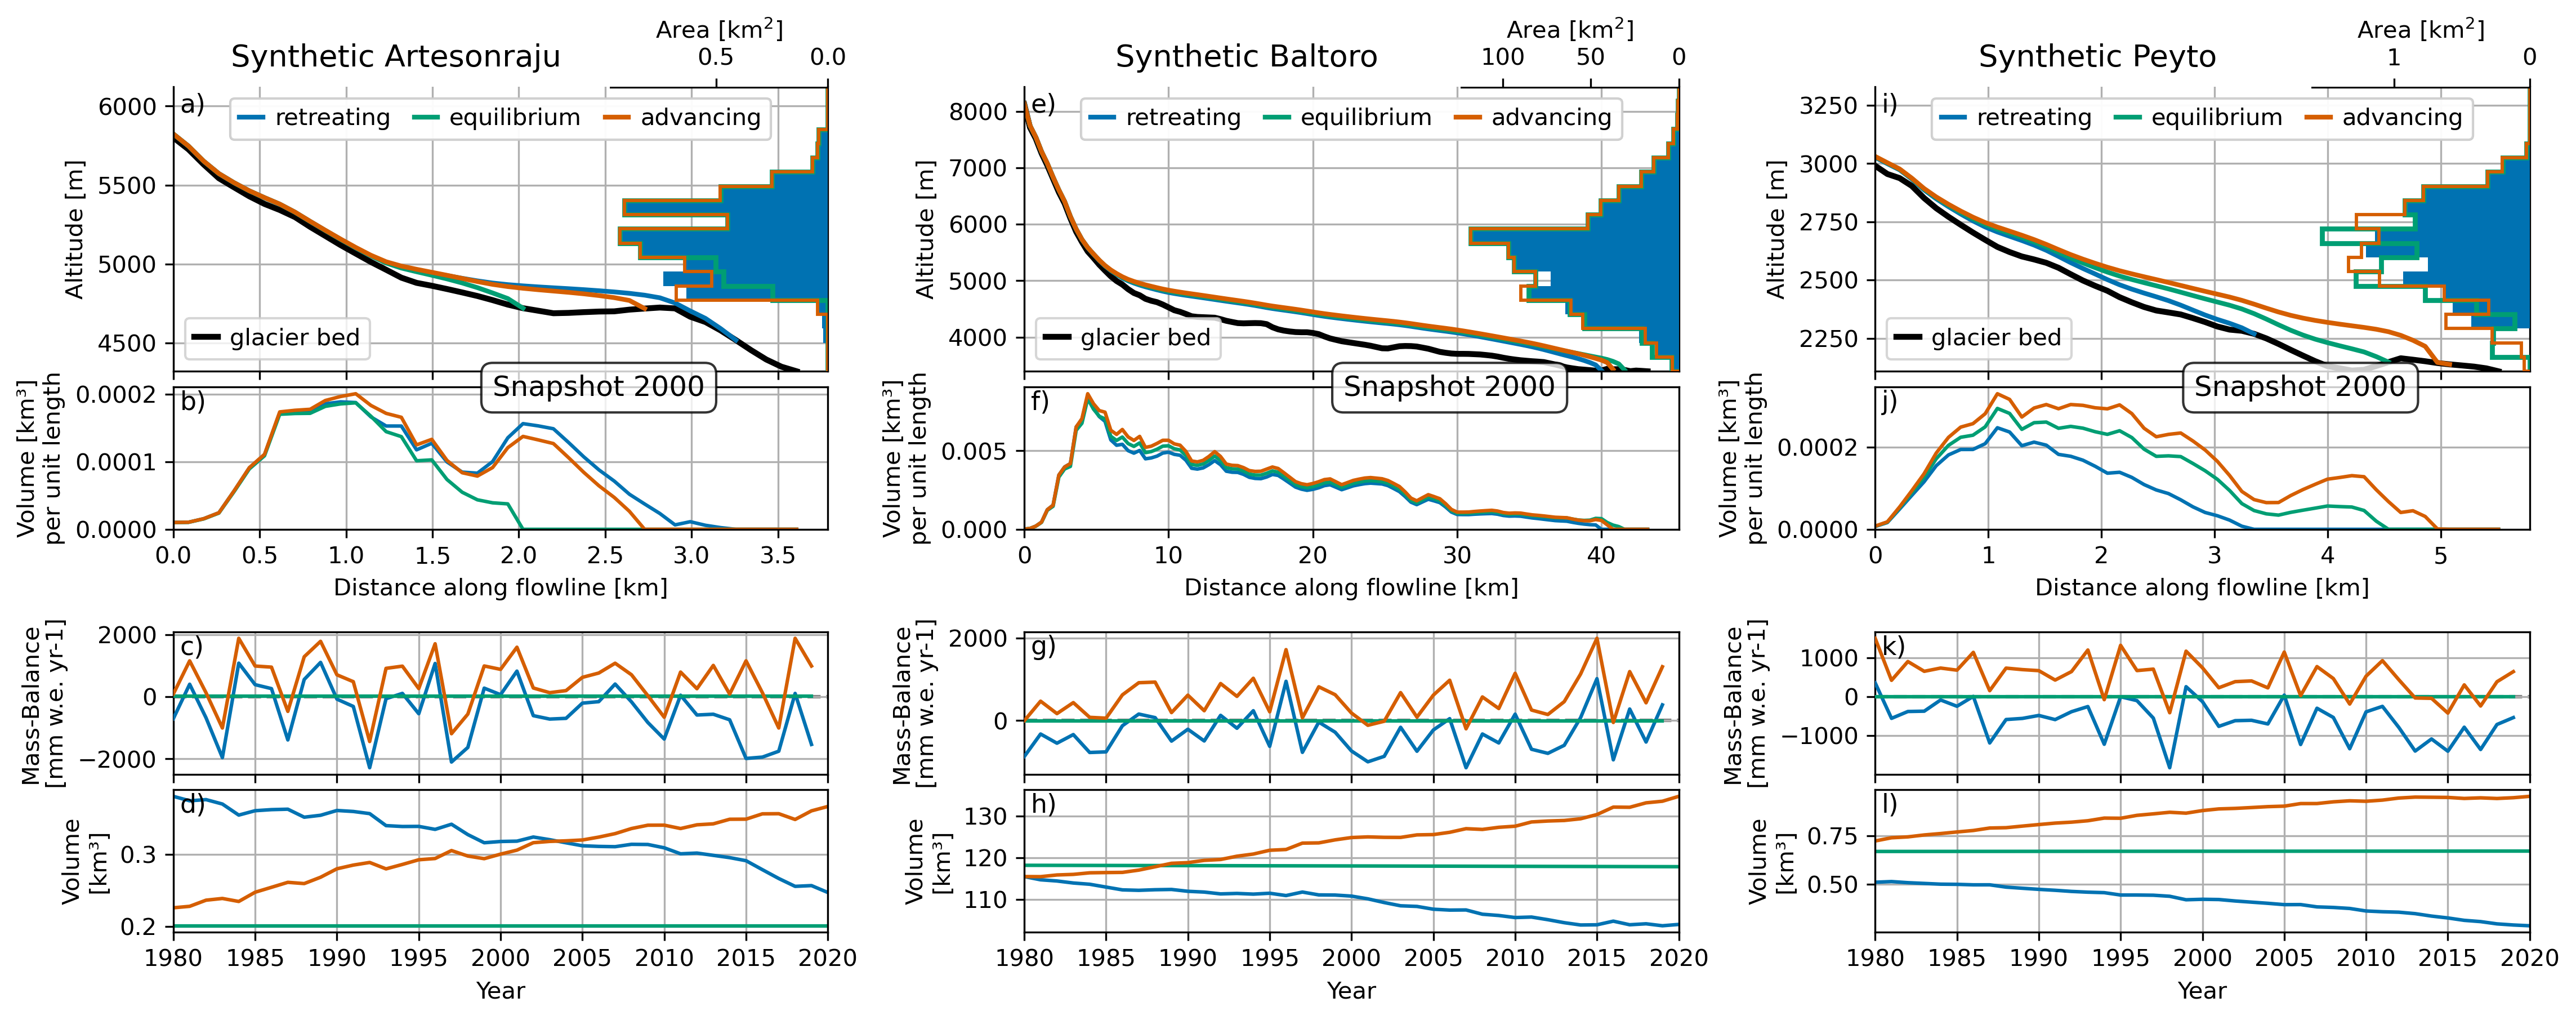
\includegraphics[width=21cm]{supfig01.png}
    \caption{Same as Figure 2 for Artesonraju (a, b, c and d), Baltoro (e, f, g and h) and Peyto (i, j, k and l).}
    \label{fig_sup:geometry_creation_artesonraju_baltoro_peyto}
\end{figure}
\end{landscape}

\received{}
\pubdiscuss{} %% only important for two-stage journals
\revised{}
\accepted{}
\published{}


\clearpage

%\bibliographystyle{copernicus}
%\bibliography{mybibfile.bib}

\end{document}
